% !TEX TS-program = pdflatexmk
\documentclass{styles/assisi}
\DeclareRobustCommand{\DelivNumber}{Multi-zone model configuration}
\DeclareRobustCommand{\DelivName}{\today}
\DeclareRobustCommand{\DelivStatus}{Confidential}
\DeclareRobustCommand{\DelivRevision}{0.1}
\DeclareRobustCommand{\DeliveryDate}{}
\DeclareRobustCommand{\DelivPartnersOwning}{\bf EPFL}
\DeclareRobustCommand{\DelivPartnersContributing}{\bf PARIS7}
\DeclareRobustCommand{\DelivPartnersContributingNextLine}{}
\DeclareRobustCommand{\DelivDue}{N/A}
\DeclareRobustCommand{\DelivAbstract}{This tutorial explains how to configure the multi-zone model in CATS2.}

%----------------------------------------------------------------------------------------------
\makeindex

\usepackage{epsfig,subfigure,float,pseudocode,multirow,footmisc,rotating}
\usepackage{graphicx}        % standard LaTeX graphics tool
\usepackage{amsmath, amssymb, subfigure}
\usepackage{multirow, rotating}
\usepackage[ruled,lined,commentsnumbered]{algorithm2e}
\usepackage[colorlinks=false, urlcolor=blue, pdfborder={0 0 0}]{hyperref}
%\usepackage{algorithm2e}
\usepackage{pdfpages}
\usepackage{afterpage}
\usepackage{booktabs}
\usepackage{geometry}
\usepackage{listings}
\usepackage{color}

\newcommand{\rd}{\Delta^{\frac{1}{2}}}
\newcommand{\pla}{\phi_{\lambda_1}^t}
\newcommand{\plb}{\phi_{\lambda_2}^t}
\newcommand{\ie}{i.\,e.,\ }
\newcommand{\Ie}{I.\,e.,\ }
\newcommand{\eg}{e.\,g.,\ }
\newcommand{\Eg}{E.\,g.,\ }
\newcommand{\assisi}{ASSISI$|_{bf}$ }
\setcounter{tocdepth}{3}

% TODO command
\newcommand{\todo}[1]{\par\noindent{\raggedright\textsc{\color{red}#1}%
    \par\marginpar{{\Large\color{red}$\star$}}}}

\begin{document}
\thispagestyle{plain}
  \vspace*{0.3cm}
  \begin{center}
  {\bf \LARGE SEVENTH FRAMEWORK PROGRAMME}\\
  \vspace*{0.6cm}
  
\includegraphics[width=0.15\textwidth]{styles/7th.png}\\
  \vspace*{2.0cm}
  \bf {\large IP}\\
  \vspace*{1.0cm}
  \bf {\Huge ASSISIbf}\\
  \vspace*{.6cm}
  \bf {\it \Large Animal‌ and‌ robot‌ Societies‌ ‌Self-organise‌ and‌ Integrate‌ by‌ Social‌ Interaction‌ (bees‌ and‌ fish)‌}\\
  \vspace*{45pt}
  {\huge \bf \DelivNumber}\\
  \vspace*{12pt}
  {\Large \it \bf \DelivName}\\
  \vspace*{70pt}
  \small
  \begin{tabular}{|ll|}
    \hline &\\
    Date of preparation: \DeliveryDate & Revision: \DelivRevision\\ &\\
    Start date of project: February 1st, 2013 & Duration: 60 months\\ &\\
    Project co-ordinator: UNIGRAZ & Classification: \DelivStatus \\ &\\
    Partners: & \\
    %& \\
    ~~{\it owning:} \DelivPartnersOwning &~~{\it contributed:} \DelivPartnersContributing\\
    &\DelivPartnersContributingNextLine\\
    &\\
    Project website: & http://assisi-project.eu\\
    &\\
    \hline
  \end{tabular}
  \end{center}
%\newpage
%
%%-----------------------------------------------------------------
%\begin{center}
%\begin{tabular}{|lp{10cm}|}
%\hline &\\
%\multicolumn{2}{|c|}{\bf \Large DELIVERABLE SUMMARY SHEET} \\
%&\\
%\hline \hline
%&\\
%Project Number: & 601074\\
%&\\
%Project Acronym: & {\bf ASSISIbf}\\
%&\\
%Title:     & Animal‌ and‌ robot‌ Societies‌ ‌Self-organise‌ and‌ Integrate‌ by‌ Social‌ Interaction‌ (bees‌ and‌ fish) \\
%&\\
%\hline \hline
%&\\
%Deliverable N$^o$: & \DelivNumber\\
%&\\
%Due Date: & Project month: \DelivDue\\
%&\\
%Delivery Date: & \DeliveryDate \\
%&\\
%\hline \hline
%&\\
%\textbf{Name:} & {\bf \DelivName}\\
%&\\
%\textbf{Description:} & \DelivAbstract\\
%&\\
%&\\
%\hline \hline
%&\\
%Partners owning: & \DelivPartnersOwning \\
%&\\
%&\\
%Partners contributed: & \DelivPartnersContributing ~\DelivPartnersContributingNextLine \\
%&\\
%&\\
%Made available to: & \DelivStatus\\
%&\\
%\hline
%\end{tabular}
%\end{center}
%%}{}



%------------------------------------------------------------------



\textsf{\tableofcontents}
%\textsf{\listoffigures}
%\addcontentsline{toc}{chapter}{List of Figures}
%\textsf{\listoftables} \addcontentsline{toc}{chapter}{List
%of Tables}

\lstset{
    language=xml,
    tabsize=3,
    %frame=lines,
    %caption=Test,
    %label=code:sample,
    %frame=shadowbox,
    %rulesepcolor=\color{gray},
    xleftmargin=20pt,
    framexleftmargin=15pt,
    %keywordstyle=\color{blue}\bf,
    %commentstyle=\color{OliveGreen},
    %stringstyle=\color{red},
    numbers=left,
    numberstyle=\tiny,
    numbersep=5pt,
    breaklines=true,
    showstringspaces=false,
    basicstyle=\footnotesize}

\chapter{Introduction}\label{chap:intro}
The multi-zone fish model provides a way to represent animals behavior that 
can vary in different areas of the experimental setup. CATS2 provides the interface to the model in the control mode {\it Zone based model}.

In this tutorial we will show how to properly setup the zone-based model in the configuration file. As as example, we will use the {\it cats2-epfl-setup.xml} configuration file, that is in the {\it config} folder in CATS2.

\chapter{Model configuration}\label{chap:intro}
\section{Install the setup}
Carefully install the experimental setup, it should not be moved later. 

\section{Define the setup map file}
The {\it xml} file with the setup map is to be copied into the {\it config/setup} folder. As an example of the setup map have a look on the {\it epfl-two-rooms.xml}. It's recommended to place the print screen with the setup into  {\it config/setup} folder, with the same name as the setup map file, e.g. {\it epfl-two-rooms.png}. The polygon defining the setup is a sequence of pairs {\it x y} specifying polygon vertices in the contre-clock-wise order in {\bf world coordinates} (listing \ref{lst:setup-map-file}). 

\begin{lstlisting}[caption={Setup map example from {\it epfl-two-rooms.xml}},label={lst:setup-map-file},language=xml]
<polygon>
   -0.34 -0.26 -0.30 -0.295
   0.005 -0.285 0.04 -0.24
   0.035 0.01 0.2 0.185
   0.45 0.195 0.485 0.23
   0.475 0.52 0.435 0.56
   0.145 0.55 0.11 0.50
   0.11 0.26 -0.06 0.09
   -0.325 0.08 -0.35 0.05
</polygon>
<excludedPolygons>
</excludedPolygons>
\end{lstlisting}

In the CATS2 configuration file the setup map is defined under {\it experiment/setupMapPath}. 
Once set it will be automatically shown in CATS2. 

\begin{figure}[ht]
\centering
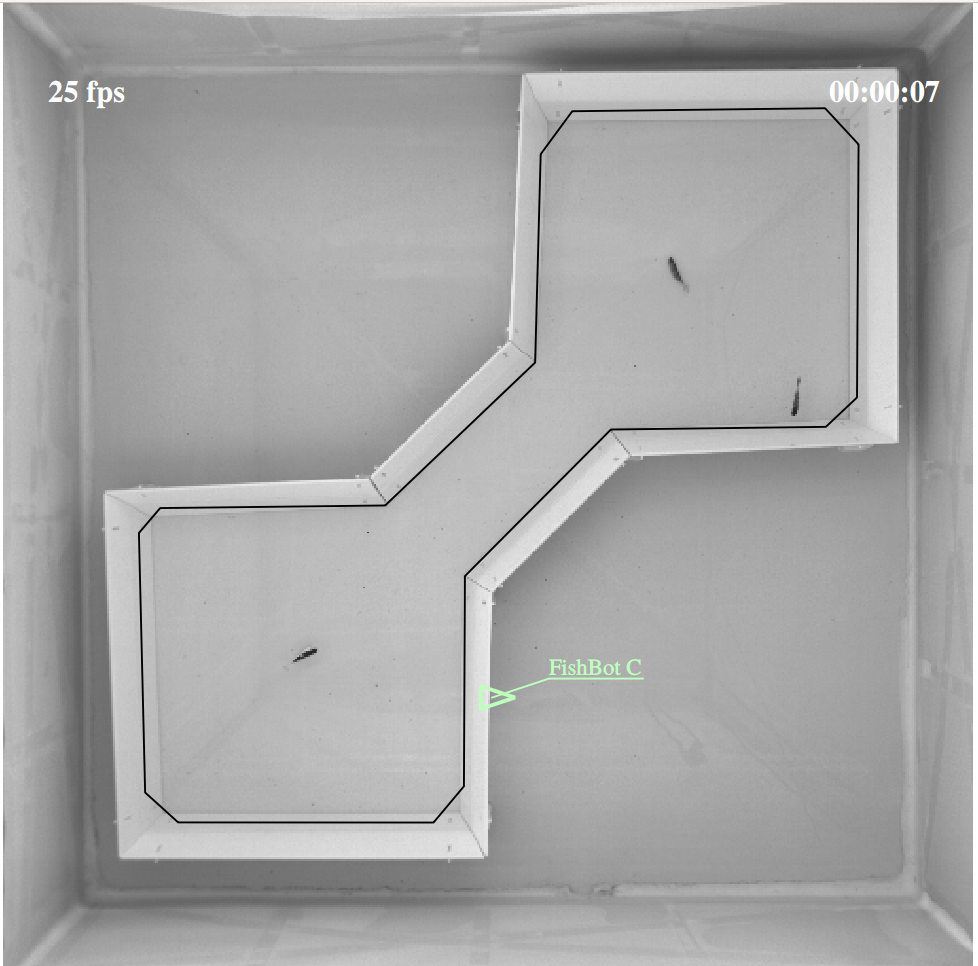
\includegraphics[width=0.5\textwidth]{./figs/setup-map.png}
\caption{The main view of CATS2 with the setup map shown above the fish two-rooms setup.}
\label{fig:setup-map}
\end{figure}

\section{Define the zones in the control map}
At the moment there is no way to visualize the zones defined in the model, and thus we will need an additional step to properly define the zones. 

\subsection{Outline the zones (optional)}
If the zones structure is complicated then print the setup print screen and manually draw the zones on it with the color pens or pencils, it will make the further work simpler.

\subsection{Create the control map}
The control map files are stored in the {\it config/control-maps} folder. For the reference check {\it epfl-two-rooms-control-map.xml}. One section of the configuration file is shown on \ref{lst:control-map}. Here we use the control map only to visualize the zones, hence the {\it id}, {\it type}, {\it controlMode} and {\it motionPattern} parameters are not important\footnote{Just note the at the moment only two types are supported: {\it room} and {\it corridor}, they are hard-coded in CATS2 that is not optimal}. One only need to set {\it polygons} and {\it color}.

\begin{lstlisting}[caption={Control map area example},label={lst:control-map},language=xml]
<area_1>
    <id>bottom</id>
    <type>room</type>
    <polygons>
        <numberOfPolygons>1</numberOfPolygons>
        <polygon_1>
            -0.33 -0.3 0.04 -0.285 0.035 0.01 -0.06 0.09 -0.35 0.08
        </polygon_1>
    </polygons>
    <color>
        <r>45</r>
        <g>130</g>
        <b>220</b>
    </color>
    <controlMode>goStraight</controlMode>
    <motionPattern>pidController</motionPattern>
</area_1>
\end{lstlisting}

Once the control map file is done, it should be set in the configuration file at {\it robots/controllers/controlMap/controlAreasPath} and then to see the zones in CATS2 one can simply activate the {\it Control map} experiment. 

\begin{figure}[ht]
\centering
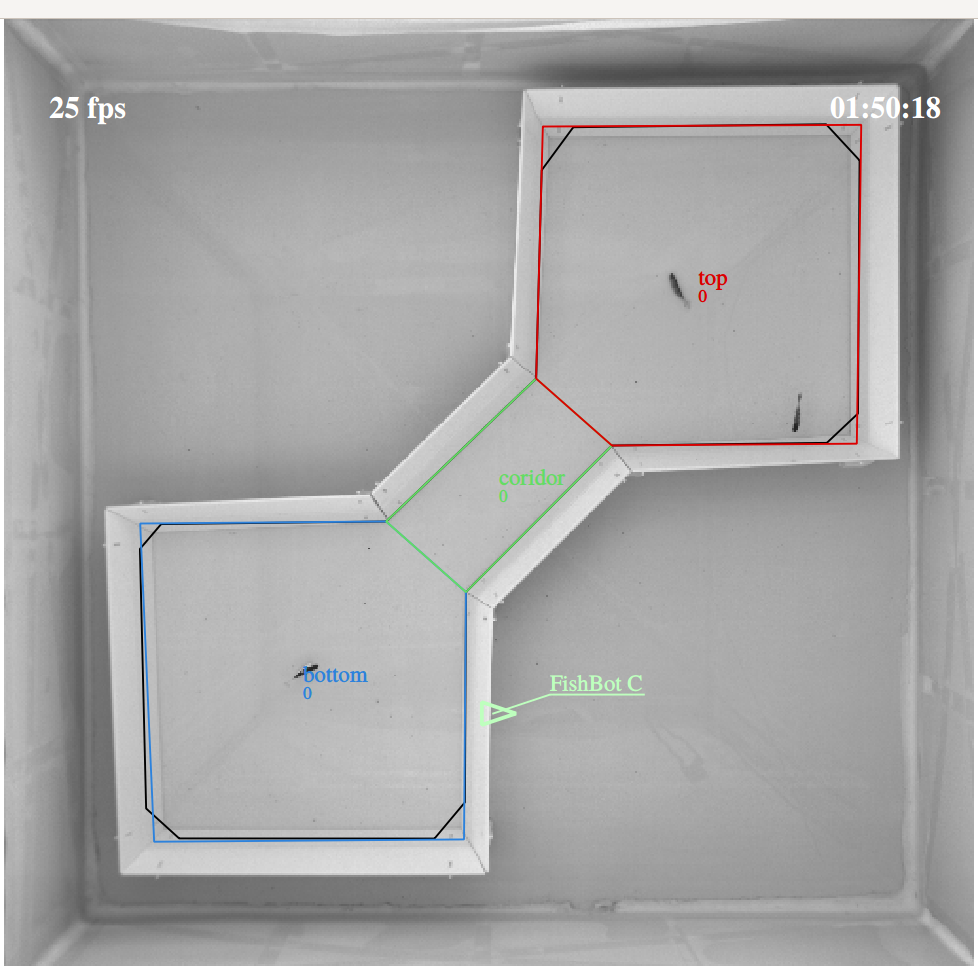
\includegraphics[width=0.5\textwidth]{./figs/control-map.png}
\caption{The main view of CATS2 with the control map shown above the fish two-rooms setup.}
\label{fig:control-map}
\end{figure}

\section{Set the zones in the configuration file}
The zone parameters go to the {\it robots/fishModel/ZonedBM} section in the configuration file. An example is given in the listing \ref{lst:control-map}.
The polygons are to be copied from the control map that we have done earlier.

\begin{lstlisting}[caption={Control map area example},label={lst:model},language=xml]
<zone_1>
    <polygons>
        <numberOfPolygons>1</numberOfPolygons>
        <polygon_1>
            -0.33 -0.3 0.04 -0.285 0.035 0.01 -0.06 0.09 -0.35 0.08
        </polygon_1>
    </polygons>
    <kappaFishes>20.0</kappaFishes>
    <alphasCenter>55.0</alphasCenter>
    <kappaNeutCenter>6.3</kappaNeutCenter>
    <repulsionFromAgentsAtDist>0.02</repulsionFromAgentsAtDist>
    <minSpeed>0</minSpeed>
    <maxSpeed>0.20</maxSpeed>
    <gammaZone>55.0</gammaZone>
    <beta>55.0</beta>
    <kappaWalls>20.0</kappaWalls>
    <speedHistogram>
        0.0304615 0.07993734 0.10186769 0.12054464 0.14286059
        0.15312688 0.14098084 0.10748283 0.07632245 0.04641523
    </speedHistogram>
    <zonesAffinity>
        0.88439782 0.99330759 0.07004122 0.01663702 0.08520822
    </zonesAffinity>
    <followWalls>0</followWalls>
</zone_1>
\end{lstlisting}

\end{document}

